\documentclass[12pt]{article}

\usepackage{fullpage}
\usepackage{multicol,multirow}
\usepackage{tabularx}
\usepackage{listings}
\usepackage[utf8]{inputenc}
\usepackage[russian]{babel}
\usepackage{graphicx}
\usepackage{csquotes}

\begin{document}

\begin{titlepage}

    \begin{center}

        \bfseries
        {\small Московский авиационный институт\\ 
        (национальный исследовательский университет)}

        % \vspace{48pt}
        {\small Факультет информационных технологий и прикладной 
        математики}
        
        % \vspace{36pt}
        {\small Кафедра вычислительной математики и программирования}
        
        \vspace{8cm}
        {\Large Лабораторная работа \textnumero 4 по курсу} 
        \enquote{\Large Компьютерная графика}
        
    \end{center}
    
    \vspace{84pt}
    \begin{flushright}
        \begin{tabular}{rl}
            Студент: & Е.Ю. Юрков \\
            % Преподаватель: &  \\
            Группа: & М80-312Б-22 \\
            Дата: & \\
            Оценка: & \\
            Подпись: & \\
        \end{tabular}
    \end{flushright}
    
    \vfill
    
    \begin{center}
        
        \bfseries
        Москва, \the\year
    
    \end{center}

\end{titlepage}

% Выполнил студент группы М8О-312Б-22 МАИ \textit{Юрков Евгений}.

\subsection*{Цель лабораторной работы}

В этой лабораторной работе вы научитесь работать с освещением в 3D-пространстве,
используя различные типы источников света, и освоите основы написания шейдеров. Вы
реализуете освещение объектов в сцене с использованием простейших моделей
освещения и настроите эффекты при помощи вершинных и фрагментных шейдеров.

\subsection*{Задача}

\textbf{Вариант 7. Использование нормальных карт для создания детализации}

Постройте куб и примените к нему текстуру.
Реализуйте нормальные карты (normal mapping) для добавления детализации на
поверхности куба без увеличения количества полигонов.
Используйте фрагментный шейдер для расчета освещения с учетом нормальной карты.
Дополнительно: Добавьте возможность переключения между нормальной картой и
стандартным затенением для сравнения результатов.

% \newpage
\subsection*{Метод решения}

Я написал класс куба для отрисовки его с помощью шейдера, он задавал Vertex Array со следующими элементами:
координаты расположения вершины, координаты текстуры, вектор нормали. Также в шейдер загружались две текстуры:
одна задавала цвет, а другая - нормали. В шейдере из карты нормалей извлекалась нормаль по формуле: 
$$normal = normalize(texture(normalMap, texCoord).rgb * 2.0 - 1.0)$$
Далее освещение рассчитывалось по полученной нормали с помощью модели освещения Фонга.

\subsection*{Результат работы программы}

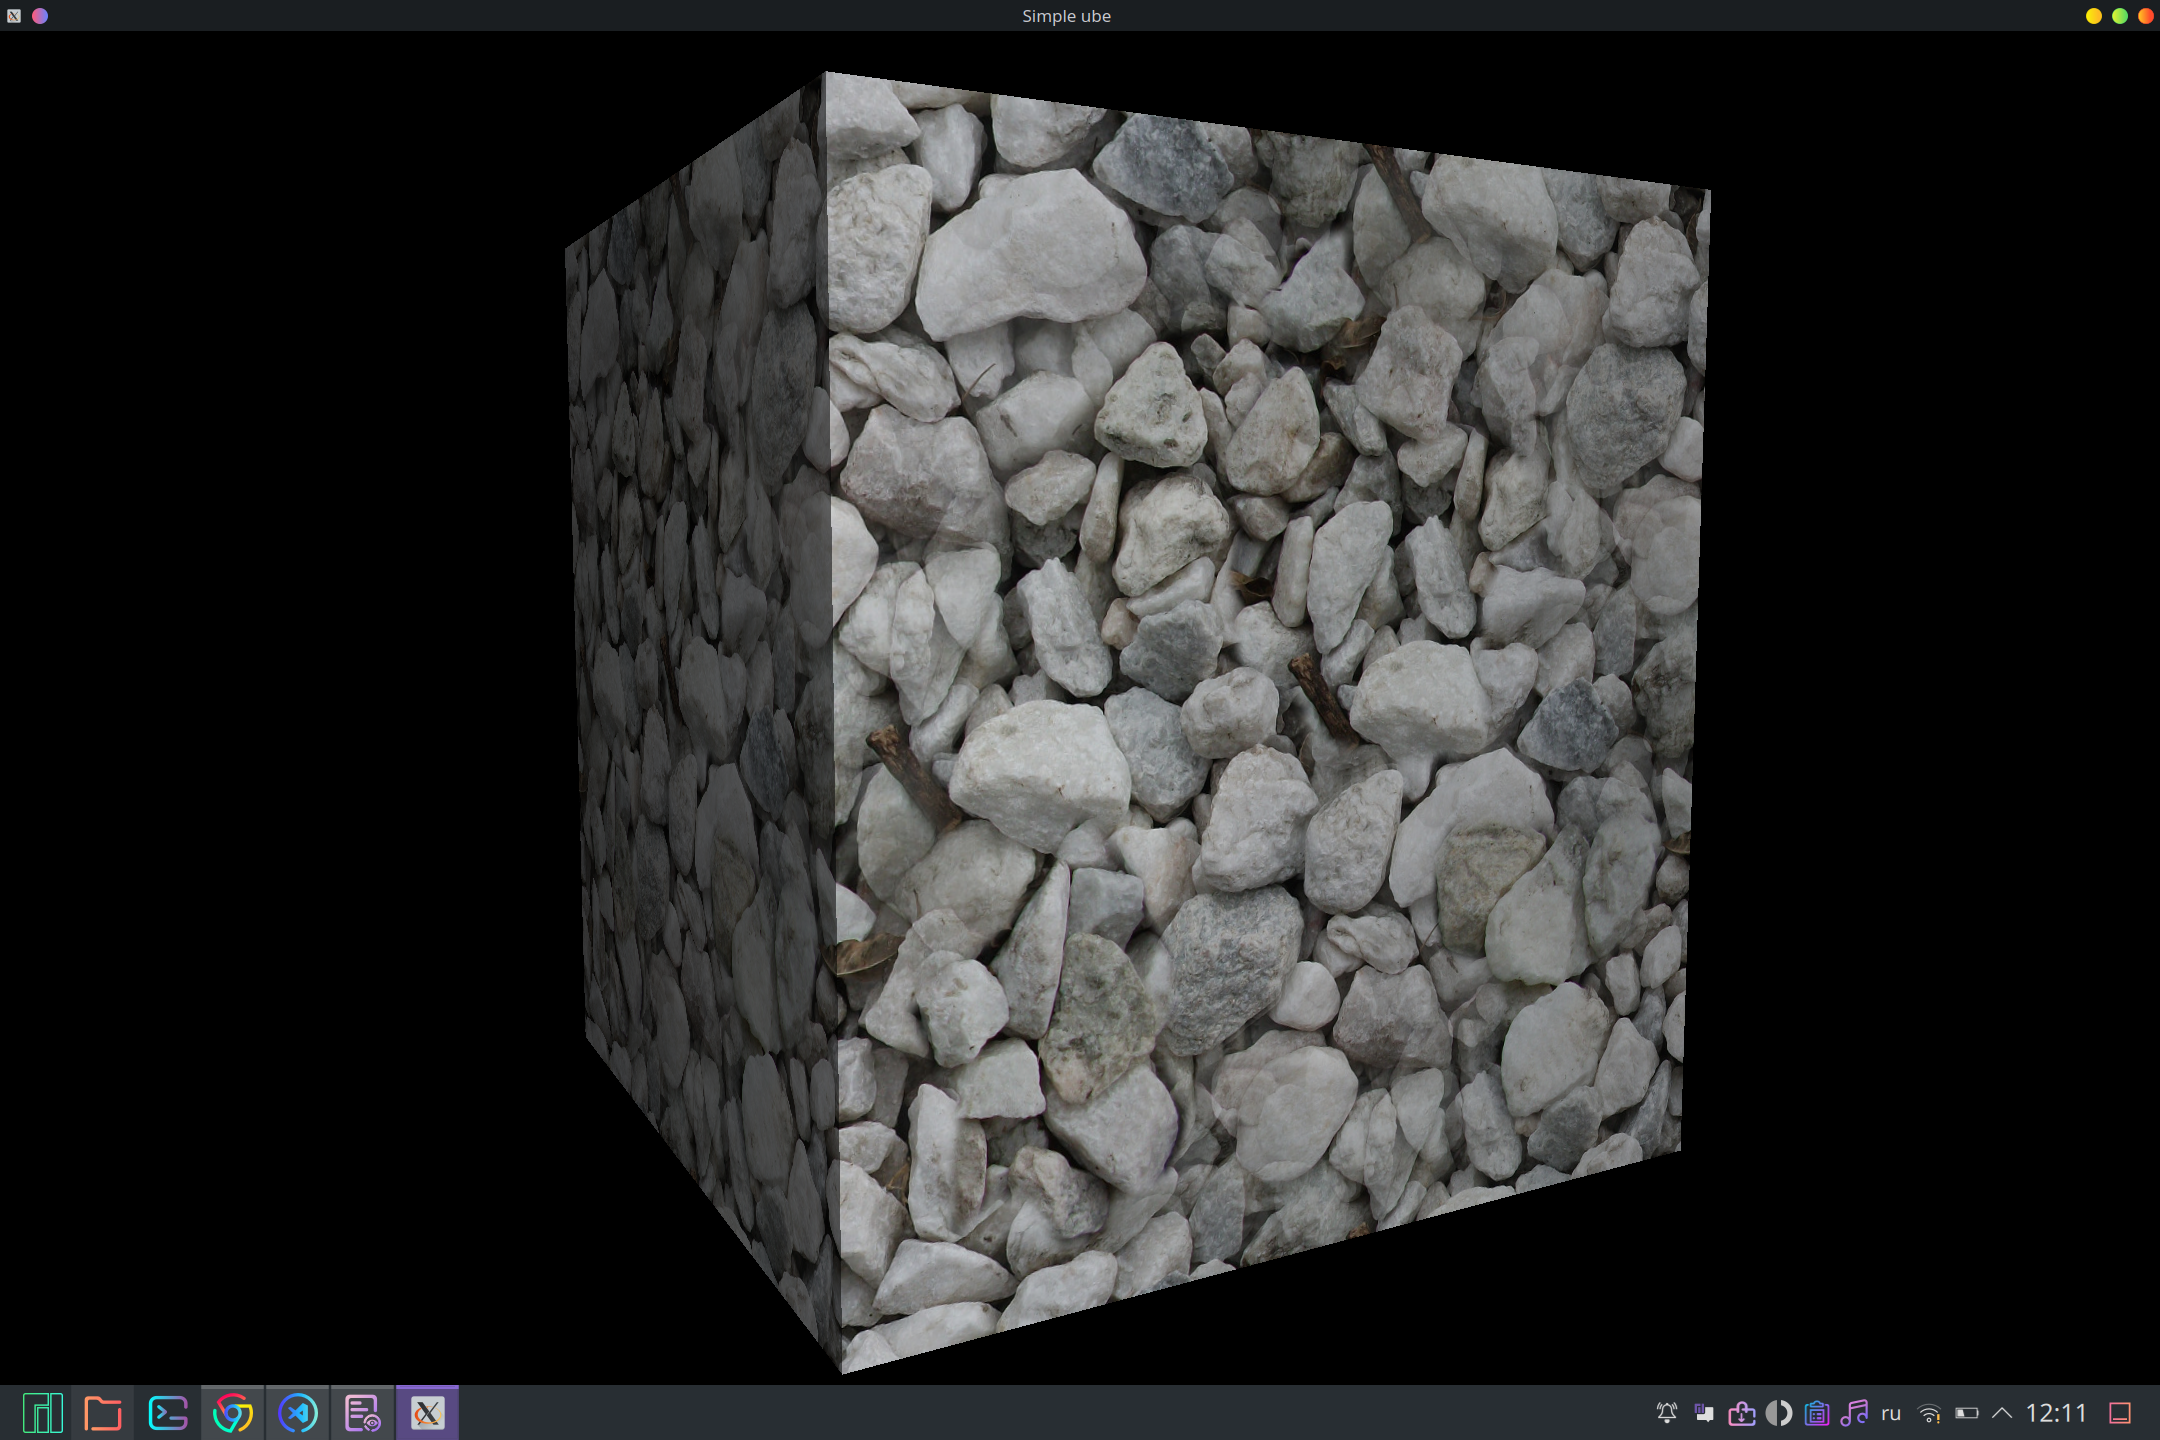
\includegraphics[width=15cm]{demo1.png} \\
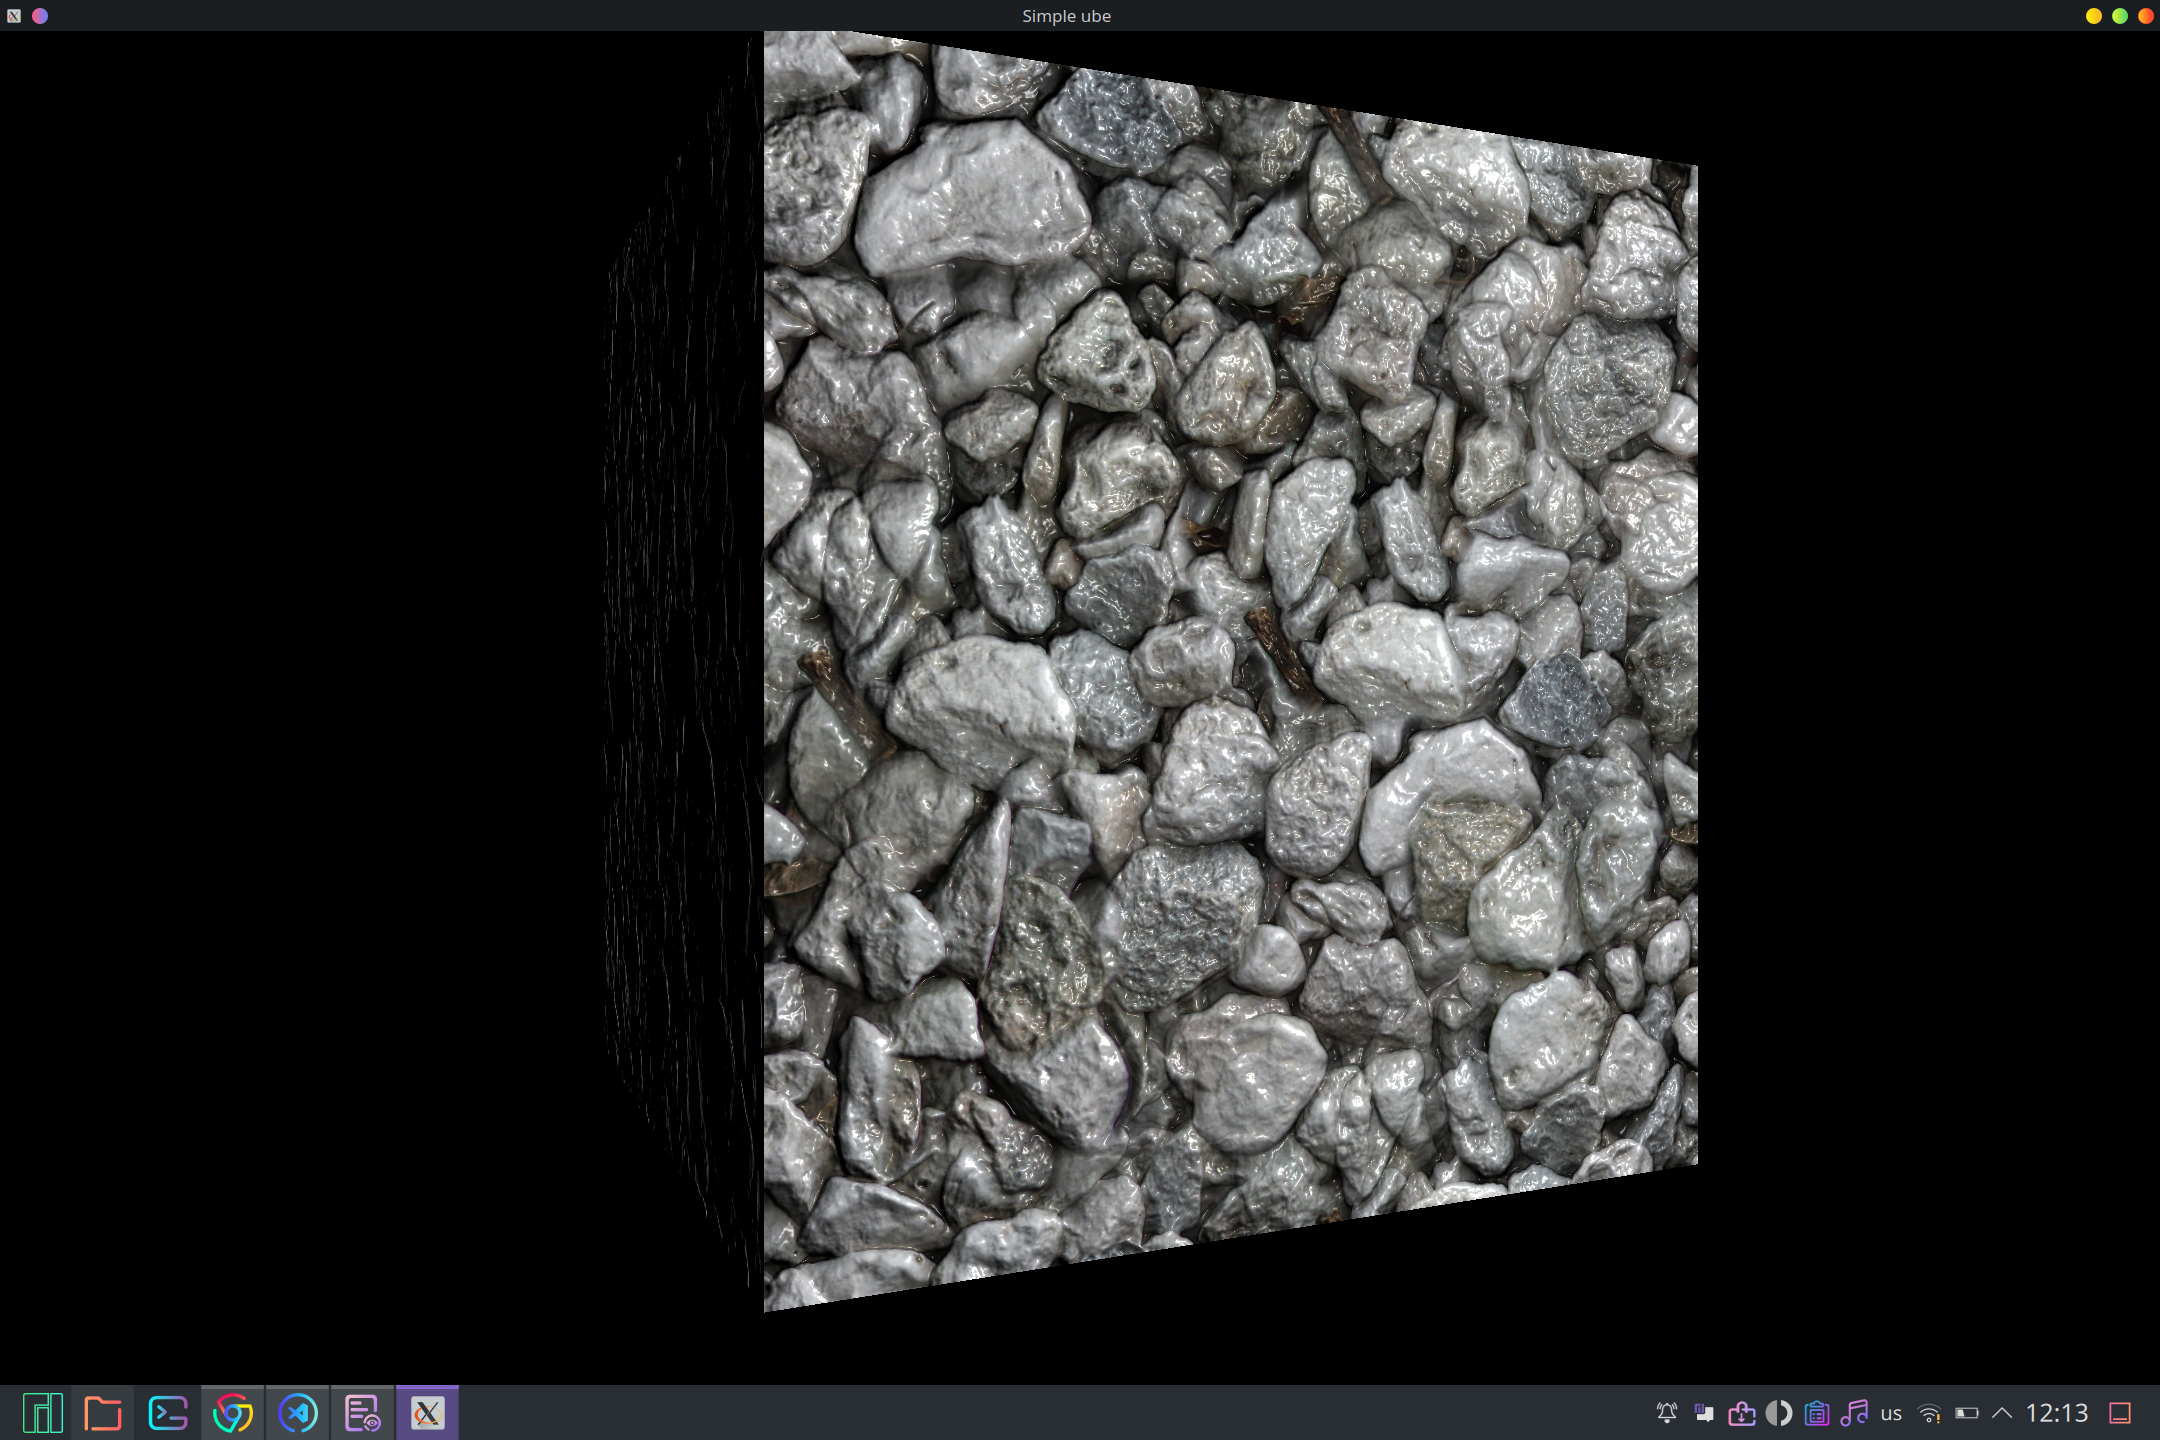
\includegraphics[width=15cm]{demo2.png}

% \newpage
\subsection*{Выводы}

В процессе выполнения лабораторной работы я узнал что такое шейдеры и научился их писать.
Я изучил, как работает освещение в компьютерной графике, в частности модель Фонга.
Также я узнал что такое карты нормалей и смог улучшить качество изображения благодаря им.

\end{document}